 \section{Segmentation}
 %MODIFIER ICI
 %%%%%%%%%%%%%%%
 % Frame Section title
 \begin{frame}
 \title{Segmentation}
 \titlepage

    \begin{minipage}{0.3\textwidth}
    \begin{flushleft} \large
    \emph{Binôme :}\\
    T. Dalens\\
    A. Dhobb
    \end{flushleft}
    \end{minipage}
    \begin{minipage}{0.5\textwidth}
    \begin{flushright} \large
    \begin{figure}
    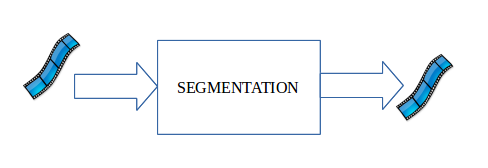
\includegraphics[width=1.4\textwidth]{Fig/architectureSectionSegmentation.png}
    \end{figure}
    \end{flushright}
    \end{minipage}\\[3cm]
    
 \end{frame}
 
 
%%%%%%%%%%%%%%%
 % Frame Architecture inpainting
\begin{frame}
  \frametitle{Architecture du programme}
  \insertF{Fig/architectureSegmentationFinale.png}{Architecture de la partie Segmentation}{0.9}
  
\end{frame} 
 
 


 %%%%%%%%%%%%%%%
 \begin{frame}
 \frametitle{Histogramme HSV}
 \insertTwoF{Fig/hsv1.jpg}{Fig/hsv2.jpg}{décomposition selon H,S et V}{0.3}
 \end{frame}
 
 \begin{frame}
 \frametitle{Histogramme HSV}
 On calcule un histogramme HSV normalisé sur 16 bins pour chaque frame : 8 bins pour H, 4 pour S et 4 pour V.\\
 \vspace{1cm}
 \verb![Rasheed, Shah, CVPR 2003]!\\
 \end{frame}
 
 \begin{frame}
 \frametitle{Détection des changements plans}
 
 \textbf{Principe :} On compare les histogrammes entre 2 frames consécutives. Si l'intersection entre ces 2 histogrammes est inférieure à un certain seuil, cela indique qu'il y a un changement de plan. \\
 \[d_{intersection}(H_{1},H_{2}) = \sum_{i} \min(H_{1}(i),H_{2}(i))\]
 
 \end{frame}
 
 
 \begin{frame}
 \frametitle{Extraction de frames clés d'un même plan}
 \textbf{Principe :}
\begin{itemize} 
\item{On fixe un deuxième seuil}
\item{On extrait la première frame du plan qui est la frame de référence}
\item{Pour chaque frame de ce plan, on calcule l'intersection de son histogramme avec l'histogramme de la frame de référence}
\item{Si l'intersection est inférieure à notre seuil, on extrait cette frame qui devient la nouvelle frame de référence}
\end{itemize}
\end{frame}

\begin{frame}
 \frametitle{Extraction de frames clés d'un même plan}
 \insertF{Fig/Spiderman.jpg}{Frames clés d'un plan de \emph{Spiderman 2}}{1}
\end{frame}


%%%%%%%%%%%%%%%%
\begin{frame}
 \frametitle{Films en noir et blanc}
 Films en noir et blanc :
 \begin{enumerate}
 \item Méthode similaire
 \item Histogramme une dimension, niveau de gris, 8 cases
 \item Résultats comparables mais inférieurs
  \insertTwoF{Fig/ldv0037-0000.jpg}{Fig/ldv0039-0001.jpg}{Extraits de \emph{La Dolce Vita}}{0.4}
 \end{enumerate}
 \end{frame}

\begin{frame}
\frametitle{Sélection des bonnes séquences}
Première idée : détecter les visages
  \insertTwoF{Fig/stark.jpg}{Fig/statue.jpg}{Extraits de \emph{The Fellowship of the Ring}}{0.6}

\end{frame}

\begin{frame}
\frametitle{Sélection des bonnes séquences}
Première idée : détecter les visages
  \insertTwoF{Fig/twd1.jpg}{Fig/twd2.jpg}{Extraits de \emph{The Walking Dead}}{0.5}

\end{frame}

\begin{frame}
\frametitle{Sélection des bonnes séquences}
Méthode : détecteur en cascade de Haar
\begin{enumerate}
\item Fonctionne sur l'image intégrale
\item Calcul de différences sur cette image
\item Entraînement des différents "patchs" avec AdaBoost
  \insertF{Fig/haarfeatures.png}{"patchs" pour la méthode de Haar}{0.5}

\end{enumerate}

\end{frame}

\begin{frame}
\frametitle{Sélection des bonnes séquences}
Deuxième idée : estimation du flou \\
Méthode : convolution avec un Laplacien
  \insertTwoF{Fig/lvd1.jpg}{Fig/lvd2.jpg}{Images floues de \emph{A Perfect World}}{0.4}
\end{frame}

\begin{frame}
\frametitle{Sélection des bonnes séquences}
Deuxième idée : estimation du flou \\
Méthode : convolution avec un Laplacien \\
Puis on regarde la netteté des points

  \insertTwoF{Fig/lvd3.jpg}{Fig/lvd4.jpg}{Images de \emph{A Perfect World}. A gauche, le score de netteté est plus élevé qu'à droite.}{0.4}
\end{frame}

\begin{frame}
\frametitle{Sélection des bonnes séquences}
Deuxième idée : estimation du flou \\
Méthode : convolution avec un Laplacien \\
Puis on regarde la netteté des points

  \insertTwoF{Fig/lvd3a.png}{Fig/lvd4a.png}{Convolution avec le Laplacien.}{0.47}
\end{frame}
\begin{frame}
\frametitle{Regroupement des séquences}
Idée : plusieurs plans peuvent être de la même scène \\
Méthode : On compare les histogrammes des plans successifs
\insertTwoF{Fig/lvd5.jpg}{Fig/lvd6.jpg}{Deux plans de \emph{A Perfect World}}{0.4}
\end{frame}


 %%%%%%%%%%%%%%%
  % Frame demonstration
 \begin{frame}
   \frametitle{Démonstration}
   \begin{figure}
   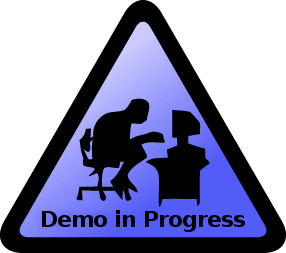
\includegraphics[width=0.5\textwidth]{Fig/demoInProgress.png}
   \end{figure}

 \end{frame}